In table \ref{glove-multiplication} the results of the GloVe method combined with the multiplication method are shown. The results for the addition method are displayed in table \ref{glove-addition}. The results of multiplication- and addition model of Word2Vec can respectively be found in table \ref{table:word2vec_multiplication} and table \ref{table:word2vec_addition}. A graph that visualizes the results next to each other is presented in figure \ref{fig:gloveword2veccomparison}.
\newline
No matter the dimension, GloVe always had the same amount of skipped words (all words) within a category. So we will not show the category results for these.
\label{sec:tabellen}
\begin{table}[H]
	\centering
	\subfloat[GloVe50d multiplication model (3 min runtime)  \label{table:glove150d_addition}]{
		\begin{tabular}{| l | c | r}
			\hline
			\textbf{Category} &    \textbf{Recall}\\ \hline
			Family 				& 0.62846 \\
			Gram1 adjective to adverb 	& 0.09980 \\
			Gram2 opposite 			& 0.04926 \\
			Gram3 comparative 		& 0.41366 \\
			Gram4 superlative 		& 0.17112 \\
			Gram5 present participle	& 0.29451 \\
			Gram7 past tense 		& 0.31153 \\
			Gram8 plural 			& 0.46021 \\
			Gram9 plural verbs 		& 0.25862 \\
			\textbf{Total}			& 0.14506 \\
			\textbf{Total no skipped}	& 0.29587 \\ \hline
		\end{tabular}
	}
	\hfill
	\subfloat[GloVe100d multiplication model (7 min runtime)  \label{table:glove100d_addition}]{
		\begin{tabular}{| l | c | r}
			\hline
			\textbf{Category} &    \textbf{Recall}\\ \hline
			Family 				& 0.77866 \\
			Gram1 adjective to adverb 	& 0.22883 \\
			Gram2 opposite 			& 0.15764 \\
			Gram3 comparative 		& 0.74850 \\
			Gram4 superlative 		& 0.50624 \\
			Gram5 present participle	& 0.65057 \\
			Gram7 past tense 		& 0.52821 \\
			Gram8 plural 			& 0.66667 \\
			Gram9 plural verbs 		& 0.57356 \\
			\textbf{Total}			& 0.26668 \\
			\textbf{Total no skipped}	& 0.54394 \\ \hline
		\end{tabular}
	}
	\hfill 
	\subfloat[GloVe200d multiplication model (10 min runtime)  \label{table:glove200d_multiplication}]{
		\begin{tabular}{| l | c | r}
			\hline
			\textbf{Category} &    \textbf{Recall}\\ \hline
			Family 				& 0.85178 \\
			Gram1 adjective to adverb 	& 0.25302 \\
			Gram2 opposite 			& 0.19581 \\
			Gram3 comparative 		& 0.83784 \\
			Gram4 superlative 		& 0.67162 \\
			Gram5 present participle	& 0.67045 \\
			Gram7 past tense 		& 0.60321 \\
			Gram8 plural 			& 0.76426 \\
			Gram9 plural verbs 		& 0.65172 \\
			\textbf{Total}			& 0.03531 \\
			\textbf{Total no skipped}	& 0.62273 \\ \hline
		\end{tabular}
	}
	\hfill
	\subfloat[GloVe300d multiplication model (20 min runtime)  \label{table:glove300d_multiplication}]{
		\begin{tabular}{| l | c | r}
			\hline
			\textbf{Category} &    \textbf{Recall}\\ \hline
			\textbf{Total}			& 0.32214 \\
			\textbf{Total no skipped}	& 0.65707 \\ \hline
		\end{tabular}
	}
	\caption[Results of GloVe multiplication models]
	{Results of GloVe multiplication models}
	\label{glove-multiplication}
\end{table}

\begin{table}[H]
	\centering
	\subfloat[GloVe50d addition model (3 min runtime) \label{table:glove50d_addition}]{
		\begin{tabular}{| l | c | r}
			\hline
			\textbf{Category} &    \textbf{Recall}\\ \hline
			Family 				& 0.85573 \\
			Gram1 adjective to adverb 	& 0.25403 \\
			Gram2 opposite 			& 0.22660 \\
			Gram3 comparative 		& 0.86486 \\
			Gram4 superlative 		& 0.69786 \\
			Gram5 present participle	& 0.68277 \\
			Gram7 past tense 		& 0.60192 \\
			Gram8 plural 			& 0.77402 \\
			Gram9 plural verbs 		& 0.59770 \\
			\textbf{Total}			& 0.30778 \\
			\textbf{Total no skipped}	& 0.62774 \\ \hline
		\end{tabular}
	}
	\hfill
	\subfloat[GloVe100d addition model (7 min runtime)   \label{table:glove100d_addition}]{
		\begin{tabular}{| l | c | r}
			\hline
			\textbf{Category} &    \textbf{Recall}\\ \hline
			Family 				& 0.81621 \\
			Gram1 adjective to adverb 	& 0.24395 \\
			Gram2 opposite 			& 0.20074 \\
			Gram3 comparative 		& 0.79129 \\
			Gram4 superlative 		& 0.54278 \\
			Gram5 present participle	& 0.69508 \\
			Gram7 past tense 		& 0.55448 \\
			Gram8 plural 			& 0.71997 \\
			Gram9 plural verbs 		& 0.58391 \\
			\textbf{Total}			& 0.28382 \\
			\textbf{Total no skipped}	& 0.57890 \\ \hline
		\end{tabular}
	}
	\hfill
	\subfloat[GloVe200d addition model (10 min runtime)   \label{table:glove200d_addition}]{
		\begin{tabular}{| l | c | r}
			\hline
			\textbf{Category} &    \textbf{Recall}\\ \hline
			Family 				& 0.85573 \\
			Gram1 adjective to adverb 	& 0.25403 \\
			Gram2 opposite 			& 0.22660 \\
			Gram3 comparative 		& 0.86486 \\
			Gram4 superlative 		& 0.69786 \\
			Gram5 present participle	& 0.68277 \\
			Gram7 past tense 		& 0.60192 \\
			Gram8 plural 			& 0.77402 \\
			Gram9 plural verbs 		& 0.59770 \\
			\textbf{Total}			& 0.30778 \\
			\textbf{Total no skipped}	& 0.62774 \\ \hline
		\end{tabular}
	}
	\hfill
	\subfloat[GloVe300d addition model (20 min runtime)    \label{table:glove300d_addition}]{
		\begin{tabular}{| l | c | r}
			\hline
			\textbf{Category} &    \textbf{Recall}\\ \hline
			\textbf{Total}				& 0.31304 \\
			\textbf{Total no skipped}	& 0.63849 \\ \hline
		\end{tabular}
	}
	\caption[Results of GloVe addition models]
	{Results of GloVe addition models}
\end{table}


\begin{table}[H]
	\centering
	\subfloat[Word2Vec multiplication model (3h25m runtime)  \label{table:word2vec_multiplication}]{
		\begin{tabular}{| l | c | r}
			\hline
			\textbf{Category} 			&    \textbf{Recall}\\ \hline
			Capital common countries 		& 0.85178 \\
			Capital World 				& 0.80570 \\
			Currency					& 0.35450 \\
			City in state				& 0.71423 \\
			Family 					& 0.84585 \\
			Gram1 adjective to adverb 		& 0.31552 \\
			Gram2 opposite 				& 0.42365 \\
			Gram3 comparative 			& 0.90691 \\
			Gram4 superlative 			& 0.91800 \\
			Gram5 present participle		& 0.80587 \\
			Gram6 nationality adjective 		& 0.89368 \\
			Gram7 past tense 			& 0.70641 \\
			Gram8 plural 				& 0.89940 \\
			Gram9 plural verbs 			& 0.73448 \\
			\textbf{Total}				& 0.75148 \\ \hline
		\end{tabular}
	}
	\hfill
	\subfloat[Word2Vec addition model (1h15m runtime)  \label{table:word2vec_addition}]{
		\begin{tabular}{| l | c | r}
			\hline
			\textbf{Category}		 	&    \textbf{Recall}\\ \hline
			Capital common countries 		& 0.83202 \\
			Capital World 				& 0.79134 \\
			Currency					& 0.35104 \\
			City in state				& 0.70896 \\
			Family 					& 0.84585 \\
			Gram1 adjective to adverb 		& 0.28528 \\
			Gram2 opposite 				& 0.42734 \\
			Gram3 comparative 			& 0.90841 \\
			Gram4 superlative 			& 0.87344 \\
			Gram5 present participle		& 0.78125 \\
			Gram6 nationality adjective 		& 0.89931 \\
			Gram7 past tense 			& 0.65962 \\
			Gram8 plural 				& 0.89865 \\
			Gram9 plural verbs 			& 0.67931 \\
			\textbf{Total}				& 0.73588 \\ \hline
		\end{tabular}
	}
	\caption{Results of Word2Vec models}
	\label{word2Vec}
\end{table}

\begin{figure}[H]
	\centering
	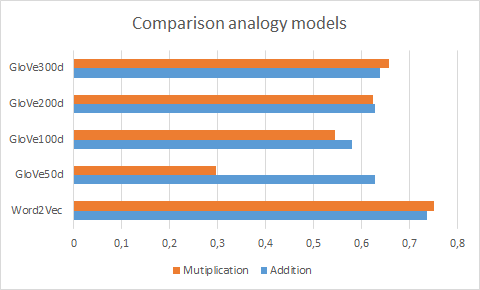
\includegraphics[width=130mm]{images/chart1.png}
	\caption{A comparison between GloVe and Word2Vec results for the multiplication and addition method.}
	\label{fig:gloveword2veccomparison}
\end{figure}